\documentclass{standalone}
\usepackage{tikz}
\usetikzlibrary{patterns, positioning}
\usepackage[sfdefault]{ClearSans} %% option 'sfdefault' activates Clear Sans as the default text font
\usepackage[T1]{fontenc}

\begin{document}
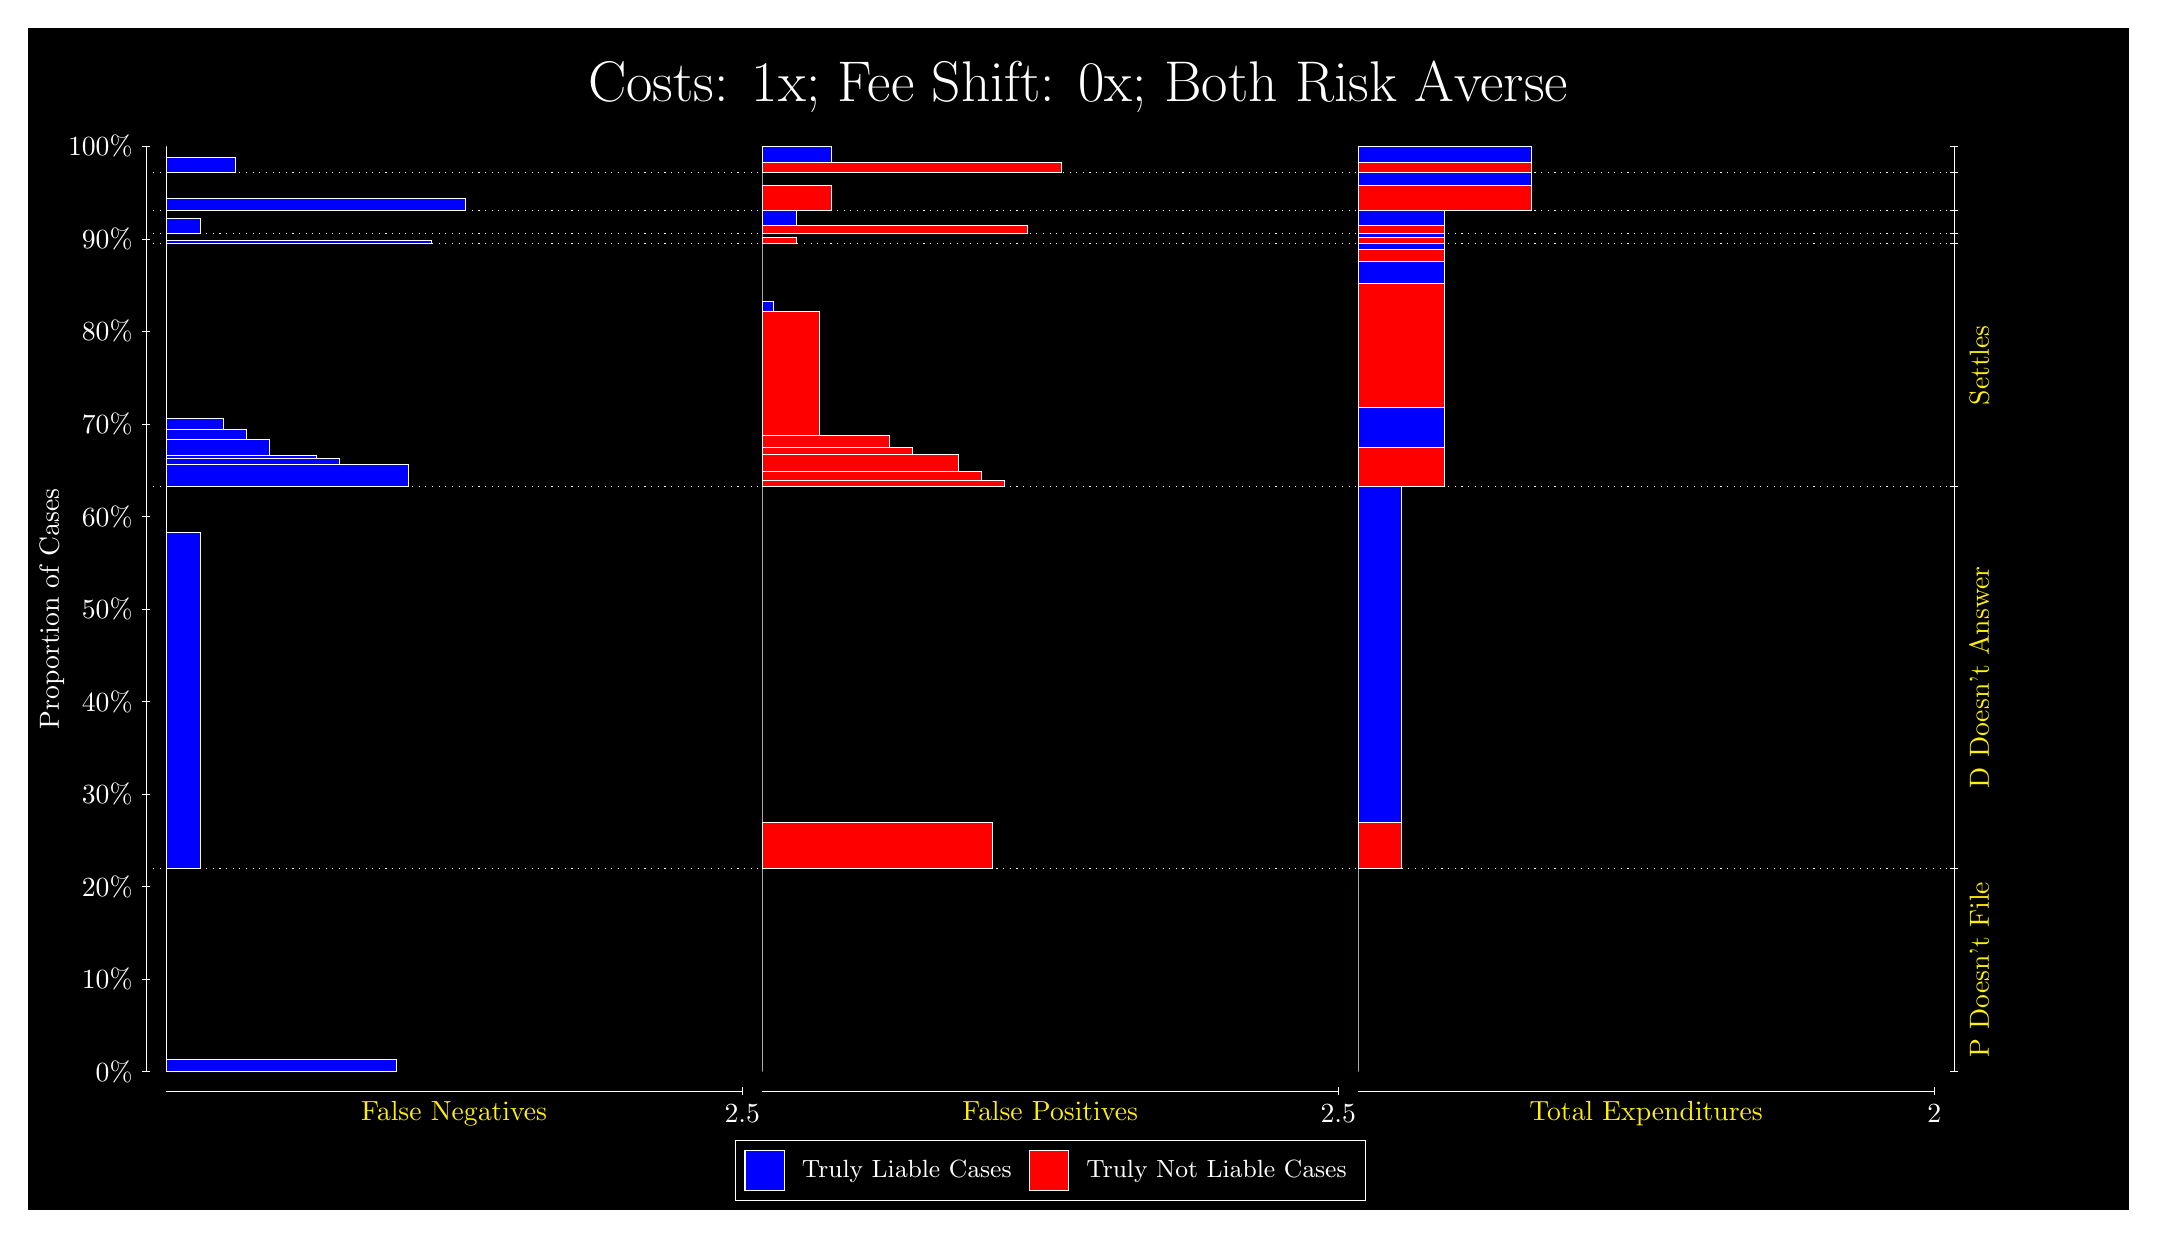
\begin{tikzpicture}
\draw[fill=black] (0,0) rectangle (26.667,15);
\draw[text=white] (0,13.5) rectangle (26.667,15) node[midway] {\huge Costs: 1x; Fee Shift: 0x; Both Risk Averse};
\draw[white, very thin] (1.5,1.75) -- (1.5,13.5);
\node[rotate=90, text=white, anchor=center] at (0.3, 7.625) {Proportion of Cases};
\draw[white, very thin] (1.45,1.75) -- (1.55,1.75);
\node[text=white, anchor=east] at (1.45, 1.75) {0\%};
\draw[white, very thin] (1.45,2.925) -- (1.55,2.925);
\node[text=white, anchor=east] at (1.45, 2.925) {10\%};
\draw[white, very thin] (1.45,4.1) -- (1.55,4.1);
\node[text=white, anchor=east] at (1.45, 4.1) {20\%};
\draw[white, very thin] (1.45,5.275) -- (1.55,5.275);
\node[text=white, anchor=east] at (1.45, 5.275) {30\%};
\draw[white, very thin] (1.45,6.45) -- (1.55,6.45);
\node[text=white, anchor=east] at (1.45, 6.45) {40\%};
\draw[white, very thin] (1.45,7.625) -- (1.55,7.625);
\node[text=white, anchor=east] at (1.45, 7.625) {50\%};
\draw[white, very thin] (1.45,8.8) -- (1.55,8.8);
\node[text=white, anchor=east] at (1.45, 8.8) {60\%};
\draw[white, very thin] (1.45,9.975) -- (1.55,9.975);
\node[text=white, anchor=east] at (1.45, 9.975) {70\%};
\draw[white, very thin] (1.45,11.15) -- (1.55,11.15);
\node[text=white, anchor=east] at (1.45, 11.15) {80\%};
\draw[white, very thin] (1.45,12.325) -- (1.55,12.325);
\node[text=white, anchor=east] at (1.45, 12.325) {90\%};
\draw[white, very thin] (1.45,13.5) -- (1.55,13.5);
\node[text=white, anchor=east] at (1.45, 13.5) {100\%};

\draw[white, very thin] (24.457,1.75) -- (24.457,13.5);
\draw[white, very thin] (24.407,1.75) -- (24.507,1.75);
\node[anchor=west] at (24.407, 1.75) {};
\draw[white, very thin] (24.407,4.3327) -- (24.507,4.3327);
\node[anchor=west] at (24.407, 4.3327) {};
\draw[white, very thin] (24.407,9.1777) -- (24.507,9.1777);
\node[anchor=west] at (24.407, 9.1777) {};
\draw[white, very thin] (24.407,12.265) -- (24.507,12.265);
\node[anchor=west] at (24.407, 12.265) {};
\draw[white, very thin] (24.407,12.397) -- (24.507,12.397);
\node[anchor=west] at (24.407, 12.397) {};
\draw[white, very thin] (24.407,12.685) -- (24.507,12.685);
\node[anchor=west] at (24.407, 12.685) {};
\draw[white, very thin] (24.407,13.166) -- (24.507,13.166);
\node[anchor=west] at (24.407, 13.166) {};
\draw[white, very thin] (24.407,13.5) -- (24.507,13.5);
\node[anchor=west] at (24.407, 13.5) {};

\draw[white, very thin, fill=blue] (1.75,1.75) rectangle (4.6775,1.9106);
\draw[white, very thin, fill=red] (1.75,1.9106) rectangle (1.75,4.3327);
\draw[white, very thin, fill=blue] (1.75,4.3327) rectangle (2.1891,8.596);
\draw[white, very thin, fill=red] (1.75,8.596) rectangle (1.75,9.1777);
\draw[white, very thin, fill=blue] (1.75,9.1777) rectangle (4.8239,9.4597);
\draw[white, very thin, fill=blue] (1.75,9.4597) rectangle (3.9457,9.5322);
\draw[white, very thin, fill=blue] (1.75,9.5322) rectangle (3.6529,9.574);
\draw[white, very thin, fill=blue] (1.75,9.574) rectangle (3.0674,9.7847);
\draw[white, very thin, fill=blue] (1.75,9.7847) rectangle (2.7746,9.906);
\draw[white, very thin, fill=blue] (1.75,9.906) rectangle (2.4819,10.04);
\draw[white, very thin, fill=red] (1.75,10.04) rectangle (1.75,12.265);
\draw[white, very thin, fill=blue] (1.75,12.265) rectangle (5.1167,12.312);
\draw[white, very thin, fill=red] (1.75,12.312) rectangle (1.75,12.397);
\draw[white, very thin, fill=blue] (1.75,12.397) rectangle (2.1891,12.581);
\draw[white, very thin, fill=red] (1.75,12.581) rectangle (1.75,12.685);
\draw[white, very thin, fill=blue] (1.75,12.685) rectangle (5.5558,12.843);
\draw[white, very thin, fill=red] (1.75,12.843) rectangle (1.75,13.166);
\draw[white, very thin, fill=blue] (1.75,13.166) rectangle (2.6283,13.365);
\draw[white, very thin, fill=red] (1.75,13.365) rectangle (1.75,13.5);
\draw[white, very thin, fill=red] (9.3189,1.75) rectangle (9.3189,4.172);
\draw[white, very thin, fill=blue] (9.3189,4.172) rectangle (9.3189,4.3327);
\draw[white, very thin, fill=red] (9.3189,4.3327) rectangle (12.246,4.9144);
\draw[white, very thin, fill=blue] (9.3189,4.9144) rectangle (9.3189,9.1777);
\draw[white, very thin, fill=red] (9.3189,9.1777) rectangle (12.393,9.2534);
\draw[white, very thin, fill=red] (9.3189,9.2534) rectangle (12.1,9.3748);
\draw[white, very thin, fill=red] (9.3189,9.3748) rectangle (11.807,9.5855);
\draw[white, very thin, fill=red] (9.3189,9.5855) rectangle (11.222,9.6727);
\draw[white, very thin, fill=red] (9.3189,9.6727) rectangle (10.929,9.8241);
\draw[white, very thin, fill=red] (9.3189,9.8241) rectangle (10.051,11.402);
\draw[white, very thin, fill=blue] (9.3189,11.402) rectangle (9.4652,11.536);
\draw[white, very thin, fill=blue] (9.3189,11.536) rectangle (9.3189,12.265);
\draw[white, very thin, fill=red] (9.3189,12.265) rectangle (9.758,12.349);
\draw[white, very thin, fill=blue] (9.3189,12.349) rectangle (9.3189,12.397);
\draw[white, very thin, fill=red] (9.3189,12.397) rectangle (12.686,12.501);
\draw[white, very thin, fill=blue] (9.3189,12.501) rectangle (9.758,12.685);
\draw[white, very thin, fill=red] (9.3189,12.685) rectangle (10.197,13.009);
\draw[white, very thin, fill=blue] (9.3189,13.009) rectangle (9.3189,13.166);
\draw[white, very thin, fill=red] (9.3189,13.166) rectangle (13.125,13.301);
\draw[white, very thin, fill=blue] (9.3189,13.301) rectangle (10.197,13.5);
\draw[white, very thin, fill=red] (16.888,1.75) rectangle (16.888,4.172);
\draw[white, very thin, fill=blue] (16.888,4.172) rectangle (16.888,4.3327);
\draw[white, very thin, fill=red] (16.888,4.3327) rectangle (17.437,4.9144);
\draw[white, very thin, fill=blue] (16.888,4.9144) rectangle (17.437,9.1777);
\draw[white, very thin, fill=red] (16.888,9.1777) rectangle (17.986,9.6727);
\draw[white, very thin, fill=blue] (16.888,9.6727) rectangle (17.986,10.181);
\draw[white, very thin, fill=red] (16.888,10.181) rectangle (17.986,11.759);
\draw[white, very thin, fill=blue] (16.888,11.759) rectangle (17.986,12.041);
\draw[white, very thin, fill=red] (16.888,12.041) rectangle (17.986,12.192);
\draw[white, very thin, fill=blue] (16.888,12.192) rectangle (17.986,12.265);
\draw[white, very thin, fill=red] (16.888,12.265) rectangle (17.986,12.349);
\draw[white, very thin, fill=blue] (16.888,12.349) rectangle (17.986,12.397);
\draw[white, very thin, fill=red] (16.888,12.397) rectangle (17.986,12.501);
\draw[white, very thin, fill=blue] (16.888,12.501) rectangle (17.986,12.685);
\draw[white, very thin, fill=red] (16.888,12.685) rectangle (19.083,13.009);
\draw[white, very thin, fill=blue] (16.888,13.009) rectangle (19.083,13.166);
\draw[white, very thin, fill=red] (16.888,13.166) rectangle (19.083,13.301);
\draw[white, very thin, fill=blue] (16.888,13.301) rectangle (19.083,13.5);
\draw[white, dotted] (1.5,4.3327) -- (24.457,4.3327);
\draw[white, dotted] (1.5,9.1777) -- (24.457,9.1777);
\draw[white, dotted] (1.5,12.265) -- (24.457,12.265);
\draw[white, dotted] (1.5,12.397) -- (24.457,12.397);
\draw[white, dotted] (1.5,12.685) -- (24.457,12.685);
\draw[white, dotted] (1.5,13.166) -- (24.457,13.166);
\draw[white, very thin] (1.75,1.5) -- (9.0689,1.5);
\node[text=yellow, anchor=north] at (5.4094, 1.5) {False Negatives};
\draw[white, very thin] (9.0689,1.45) -- (9.0689,1.55);
\node[text=white, anchor=north] at (9.0689, 1.45) {2.5};

\draw[white, very thin] (9.3189,1.5) -- (16.638,1.5);
\node[text=yellow, anchor=north] at (12.978, 1.5) {False Positives};
\draw[white, very thin] (16.638,1.45) -- (16.638,1.55);
\node[text=white, anchor=north] at (16.638, 1.45) {2.5};

\draw[white, very thin] (16.888,1.5) -- (24.207,1.5);
\node[text=yellow, anchor=north] at (20.547, 1.5) {Total Expenditures};
\draw[white, very thin] (24.207,1.45) -- (24.207,1.55);
\node[text=white, anchor=north] at (24.207, 1.45) {2};

\node[text=yellow, centered, rotate=90] at (24.777, 3.0413) {P Doesn't File};
\node[text=yellow, centered, rotate=90] at (24.777, 6.7552) {D Doesn't Answer};
\node[text=yellow, centered, rotate=90] at (24.777, 10.721) {Settles};





\draw (12.978300999999998,1.5) node[draw=none] (baseCoordinate) {};
\begin{scope}[align=center]
        \matrix[scale=0.5, draw=white, below=0.5cm of baseCoordinate, nodes={draw}, column sep=0.1cm]{
            \node[rectangle, draw, minimum width=0.5cm, minimum height=0.5cm, fill=blue] {}; &
            \node[draw=none, font=\small, text=white] (B) {Truly Liable Cases}; &
            \node[rectangle, draw, minimum width=0.5cm, minimum height=0.5cm, fill=red] {}; &
            \node[draw=none, font=\small, text=white] (B) {Truly Not Liable Cases}; \\
            };
\end{scope}

\end{tikzpicture}
\end{document}